\documentclass[portrait,final,a0paper,fontscale=0.36]{baposter}

%% read in constants, custom functions and used packages

%%%%%%%%%%%%%%%%%%%%%%%%%%%%%%%%%%%%%%%%%%%%%%%%%%%%%%%%%%%%%%%%%%%%%%%% References paths
\usepackage[backend=biber, style=nature, citestyle=nature]{biblatex}
\addbibresource{ActiveSelf.bib}
% font size
\AtBeginBibliography{\scriptsize}

%%%%%%%%%%%%%%%%%%%%%%%%%%%%%%%%%%%%%%%%%%%%%%%%%%%%%%%%%%%%%%%%%%%%%%%% Image paths
\usepackage{graphicx}
\graphicspath{{logos/}{figures/}}

%%%%%%%%%%%%%%%%%%%%%%%%%%%%%%%%%%%%%%%%%%%%%%%%%%%%%%%%%%%%%%%%%%%%%%%% Color Settings
\usepackage{xcolor}
\definecolor{iftucfont}{RGB}{74,130,70}
\definecolor{iftuccolor}{RGB}{143,168,92}
\definecolor{iftucbackground}{RGB}{241,244,234}

%%%%%%%%%%%%%%%%%%%%%%%%%%%%%%%%%%%%%%%%%%%%%%%%%%%%%%%%%%%%%%%%%%%%%%%% Font Settings
\usepackage[sfdefault, regular]{roboto}

%%%%%%%%%%%%%%%%%%%%%%%%%%%%%%%%%%%%%%%%%%%%%%%%%%%%%%%%%%%%%%%%%%%%%%%% Multicol Settings
\usepackage{multirow}
\usepackage{multicol}
\setlength{\columnsep}{1.5em}
\setlength{\columnseprule}{0mm}

%% Row Settings
\usepackage{setspace}% for \onehalfspacing
\usepackage{parskip}

%% Control layout of itemize, enumerate, description
\usepackage{enumitem}

% page borders and header height
\usepackage{geometry}
\geometry{
	left=35pt,
	right=5pt,
	top=10pt
}

\newcommand{\compresslist}{% Define a command to reduce spacing within itemize/enumerate environments, e.g. \begin{itemize}\compresslist
			\setlength{\itemsep}{1pt}
			\setlength{\parskip}{0pt}
			\setlength{\parsep}{0pt}
		}
	
\newcommand{\compressbib}{%
		\setlength{\itemsep}{0pt}
		\setlength{\parskip}{0pt}
		\setlength{\parsep}{0pt}
	}
	
%%%%%%%%%%%%%%%%%%%%%%%%%%%%%%%%%%%%%%%%%%%%%%%%%%%%%%%%%%%%%%%%%%%%%%%% Table and figure settings
\usepackage{float, booktabs, array, ragged2e}

% Adjust row width in tables 
\renewcommand{\arraystretch}{1.1}

% for awesome plots and tables from files like .csv
\usepackage{pgfplots}
\usepackage{pgfplotstable}

% Graphics package-alike macros for “general” boxes. Like resizing figures and aligning minipages
\usepackage{adjustbox}

\usepackage[
font=footnotesize,
labelfont=bf,
%labelfont=sc, %Kapitälchen, passt nicht wg. nicht-osf Ziffern
%%%%labelfont=it, %italics, 
%%%labelfont=sl, %slanted,
hypcap=true,
format=hang,
%margin={2cm,2cm}
width=0.8\linewidth
]{caption}

%%%%%%%%%%%%%%%%%%%%%%%%%%%%%%%%%%%%%%%%%%%%%%%%%%%%%%%%%%%%%%%%%%%%%%%% Other packages
% to help with long equations
\usepackage{amsmath}

% for todo notes
\usepackage{todonotes} 

% for comment blocks
\usepackage{verbatim}

% link URLs
\usepackage{url}

\usepackage{lipsum}


\definecolor{loop1}{HTML}{67AB9F}
\definecolor{loop2}{HTML}{FFB570}

\definecolor{direct}{HTML}{6C8EBF}
\definecolor{indirect}{HTML}{B85450}

\setlength\bibitemsep{0.8\itemsep}

\begin{document}

\begin{poster}%
	% Poster Options
	{
		% Show grid to help with alignment
		grid=false,
		% Number of columns and column spacing
		columns=6,
		colspacing=1em,
		% Color style
		bgColorOne=white,
		borderColor=iftuccolor,
		headerColorOne=iftucbackground,
		headerFontColor=iftucfont,
		boxColorOne=white,
		% Format of textbox
		textborder=rounded,
		textfont=\small,
		% Format of text header
		eyecatcher=true,
		headerborder=closed,
		headerheight=0.1\textheight,
		%  textfont=\sc, An example of changing the text font
		headershape=rounded,
		headershade=plain,
		headerfont=\Large\bf, %Sans Serif
		% textfont={\setlength{\parindent}{1.5em}},
		boxshade=plain,
		%  background=shade-tb,
		background=plain,
		linewidth=2pt
	}
	% University logo
	{\includegraphics[height=6.5em]{tuckhseng_color}} 
	% Title
	{\bf\LARGE{The contribution of the basal ganglia in the integration of goals and  body representations: A neurocomputational study}\vspace{10pt}}
	% Authors
	{\large Erik~Syniawa and Fred~Hamker \\ \vspace{0.5em}
	
	\small \centering Contact: fred.hamker@informatik.tu-chemnitz.de \\ erik.syniawa@informatik.tu-chemnitz.de
	}
	% Department logo and other logos
	{	
		\begin{minipage}[r]{0.1\textwidth}
			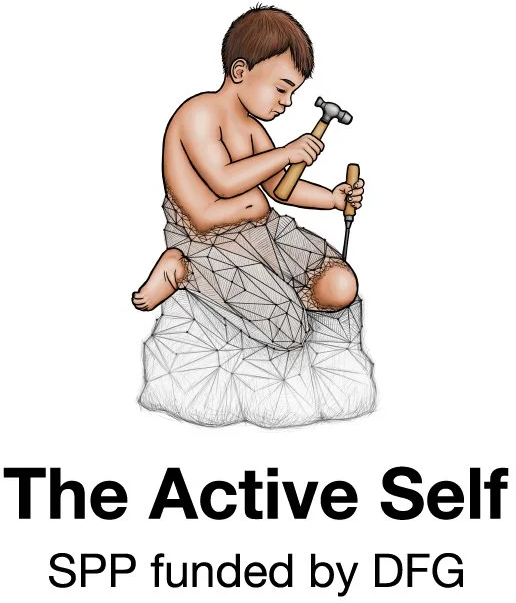
\includegraphics[height=7em]{active_self_logo_color}
		\end{minipage}
		\hfill
		\begin{minipage}[r]{0.1\textwidth}
			
\includegraphics[height=6.5em]{TUC_AI_color}
		\end{minipage}
		
	}

%%%%%%%%%%%%%%%%%%%%%%%%%%%%%%%%%%%%%%%%%%%%%%%%%%%%%%%%%%%%%%%%%%
% use height in headerbox to align multiple boxes 
% height= <size in percent of column height>, else [auto]%
\headerbox{\large Overview}{name=overview,column=0,row=0, span=3, height=0.135}{
	
	
	\begin{adjustbox}{minipage=0.95\textwidth, margin=5pt, center}
		\begin{minipage}[l]{0.35\textwidth}
			\centering
			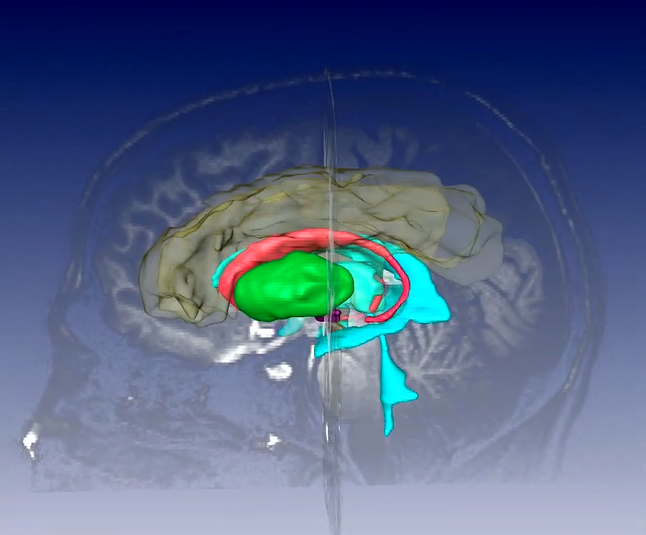
\includegraphics[width=0.7\linewidth]{BG_3D_screenshot}
			\captionof{figure}{3D Reconstruction \\of the BG \parencite{BG}.}
		\end{minipage}
		\begin{minipage}[l]{0.65\textwidth}
			\justifying
			The \textit{basal ganglia} (BG), a collection of subcortical nuclei, intricately govern motor control, learning, executive functions, and emotional behaviors. \\ 
			Through \textit{dopamine-modulated plasticity}, the BG dynamically modulate cortical input, crucial for the acquisition and execution of a diverse array of movements \parencite{parkBasalGangliaCircuits2020, dudmanBasalGangliaMotor2016}.\\ 
			Here we introduce a novel perspective on how the basal ganglia could integrate various body positions and enable the learning of motor skills.
		\end{minipage}
	\end{adjustbox}
}

\headerbox{\large Setup}{name=setup,column=3,row=0, span=3, height=0.135}{
	\begin{adjustbox}{minipage=0.95\textwidth, margin=5pt, center}
		\begin{minipage}[l]{0.5\textwidth}
			\vspace{1pt}
			
			\centering
			\includegraphics[width=0.75\linewidth]{robot_setup}
			\captionof{figure}{Current virtual robot setup.}
		\end{minipage}
		\begin{minipage}[l]{0.5\textwidth}
			\justifying
			\textbf{Task:} \\
			Based in 2D-plane a robot should touch this left forearm. He visually fixates the corresponding point on this forearm (\textcolor{red}{red point} in figure 2). \\
			The robot fixates the point it intends to touch visually. This point serves as a prediction to choose the right action from an arbitrary initial body position.
		\end{minipage}
	\end{adjustbox}
}

\headerbox{\large Computational model}{name=network, column=0, below=overview, span=3, height=0.53}{
	\begin{adjustbox}{minipage=0.95\textwidth, margin=5pt, center}
	% Network definitions
	\centering
	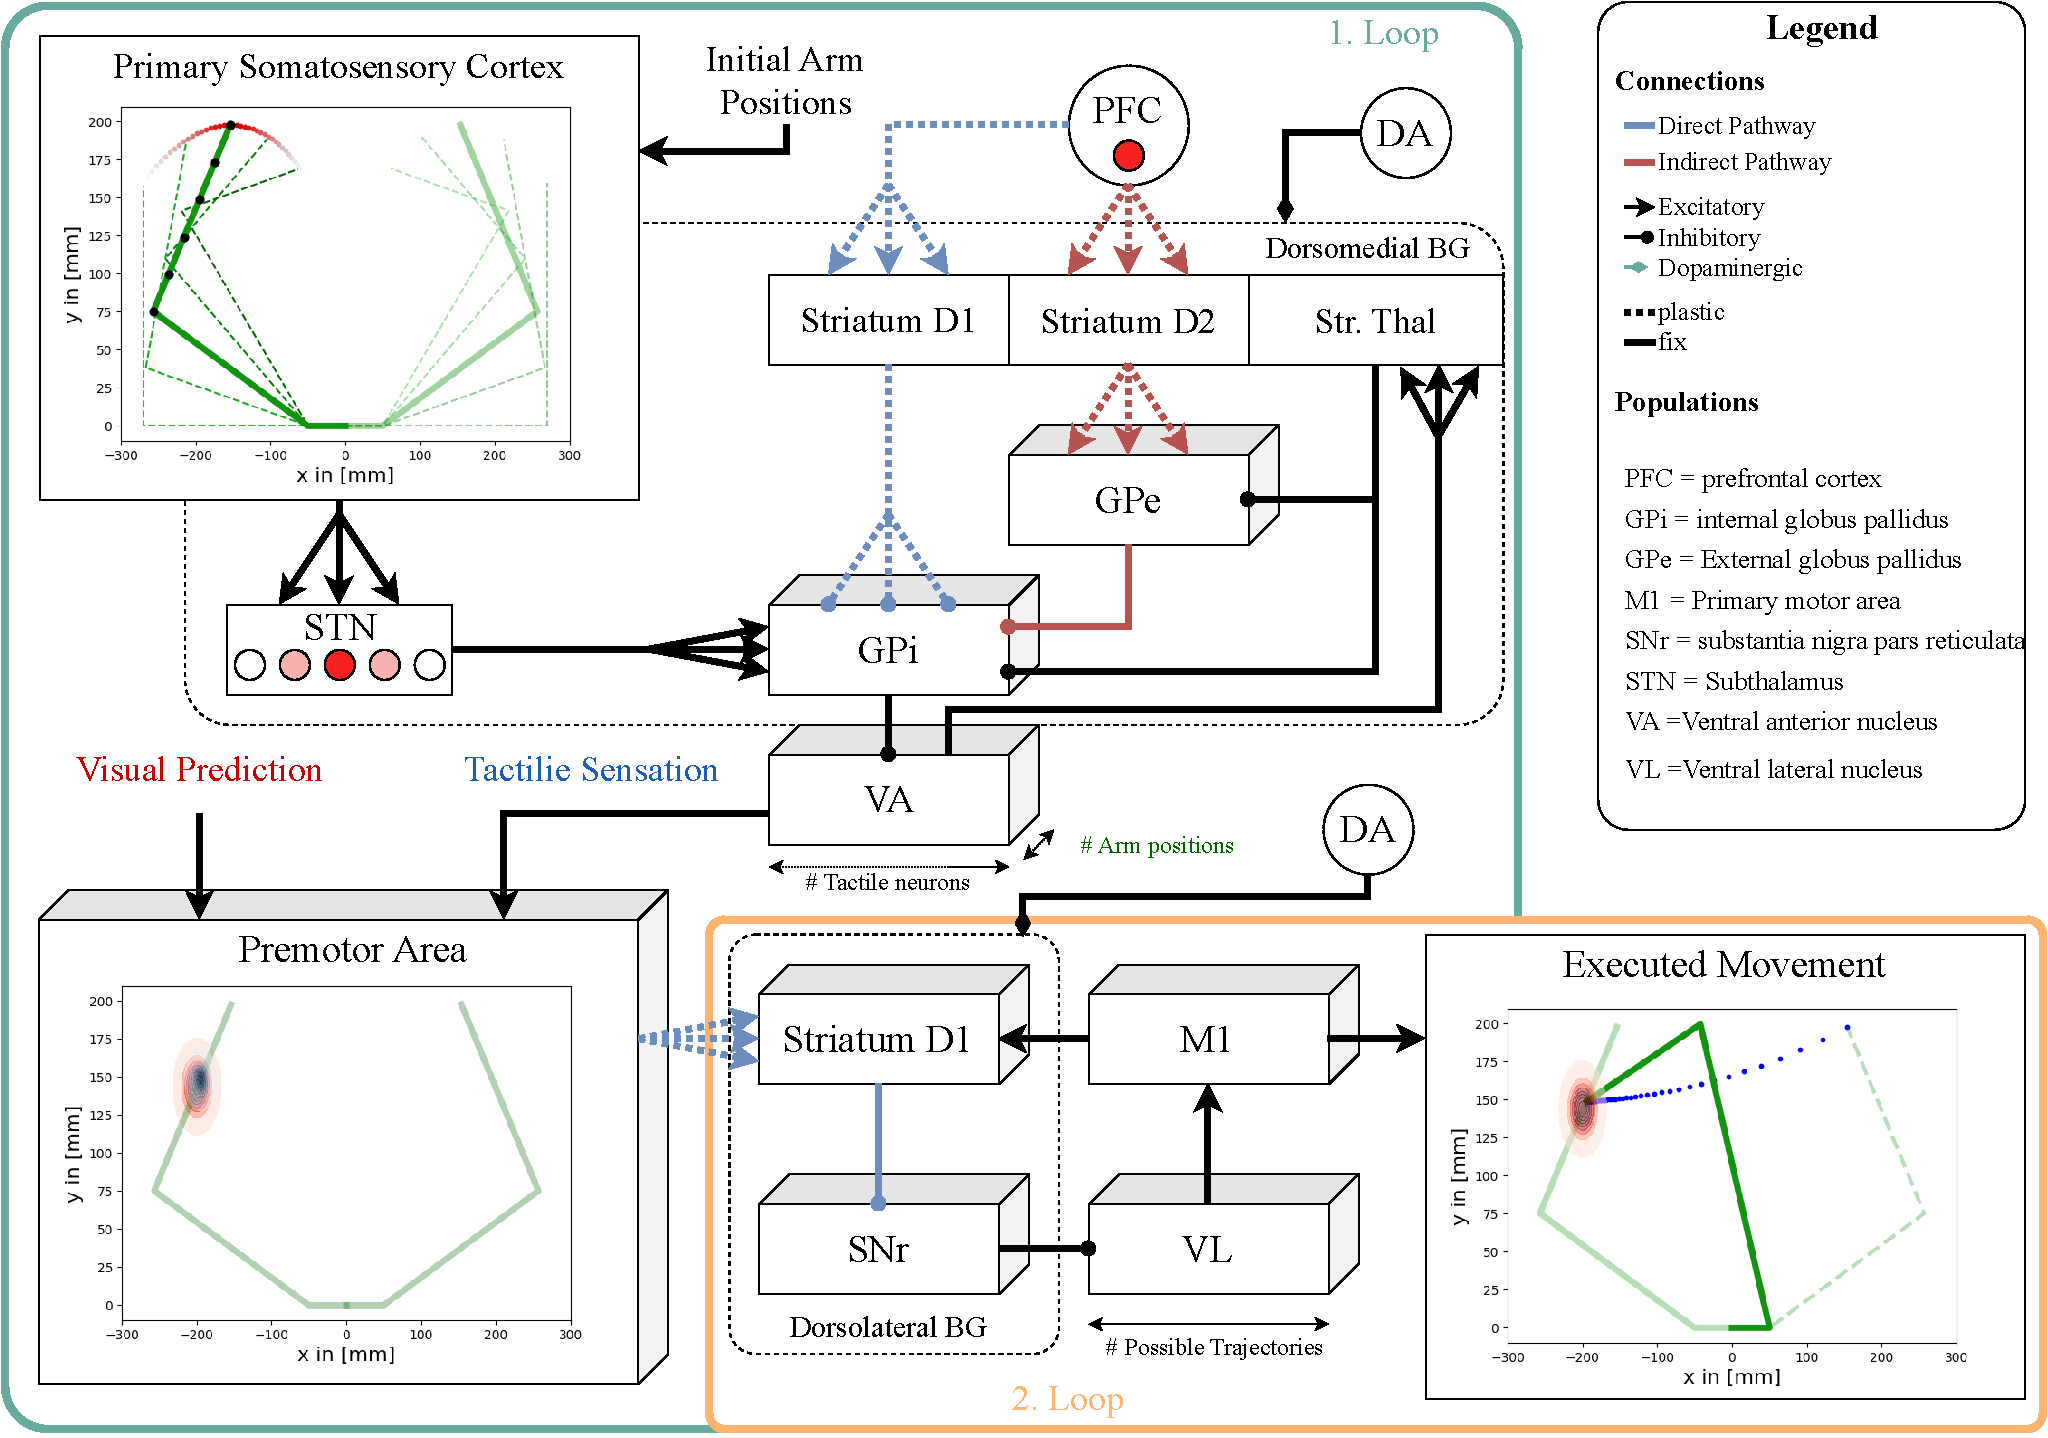
\includegraphics[width=\linewidth]{BG_inverse_model}
	\captionof{figure}{Overview of the whole model.}
	\vspace{5pt}
	\justifying	
	\begin{multicols}{2}
	Our model consist of 2 cortico-basal ganglia-thalamocortical (CBGT-) Loops (see figure 3).
	\\
	The \textcolor{loop1}{1st Loop} combines a visual goal in relation with the arm position and the  \textcolor{loop2}{2nd loop} learns an action, that is able to reach this resulting goal \parencite{baladronContributionBasalGanglia2023b}. \\
	
	The model is implemented in Python 3.11 and uses the neurosimulator ANNarchy 4.7.2.6 \parencite{vitayANNarchyCodeGeneration2015}.\\
	
	\textit{PFC:}
	\begin{itemize}[itemsep=0pt, topsep=0pt]
		\item Encodes a dimensionless intention for movement
		\item The number of neurons amount to the number of representations to be learnt
	\end{itemize}
	\textit{Primary Somatosensory Cortex (S1):}
	\begin{itemize}[itemsep=0pt, topsep=0pt]
		\item Encodes all possible arm positions (in this example 5)
		\item Only one position can be active (see figure 3 bold \textcolor{green}{green})
		\item Arm positions with nearby end effectors are also excited in the STN (in figure 3 the distance is shown in \textcolor{red}{red}) 
	\end{itemize}
	\textit{STN:}
	\begin{itemize}[itemsep=0pt, topsep=0pt]
		\item Neurons in the STN excite Neurons in the GPi, that do not correspond with active representations in the STN
	\end{itemize}
	\textit{Premotor Area:}
	\begin{itemize}[itemsep=0pt, topsep=0pt]
		\item Here, the visual goal is linked with the most active tactile neuron stimulated by VA
		\item If the positions align, a DA Signal is send to the \textcolor{loop1}{1st CBGT-Loop}
	\end{itemize}
	\textit{M1:}
	\begin{itemize}[itemsep=0pt, topsep=0pt]
		\item After one neuron exceeds a threshold a movement is executed
		\item If the executed hand position and the visual goal align a DA Signal is send to the \textcolor{loop2}{2nd CBGT-Loop}
	\end{itemize}
	
	\end{multicols}
	\end{adjustbox}
}

\headerbox{\large Model definitions}{name=plastic, column=3, below=setup, span=3, height=0.395}{
	\begin{adjustbox}{minipage=0.95\textwidth, margin=5pt, center}
		
		\begin{minipage}[l]{0.47\textwidth}
			\textbf{Learning in the different pathways:}\\
			\justifying
			
			The learning principles are primarily determined by \textit{pre-} and \textit{post-synaptic} activity, as well as the \textit{DA-Signal}. Together these principles form a 3-factor learning rule (see Table 1, modified after \cite{maithOptimalAttentionTuning2021c}).
			\vspace{1pt}
			\begin{itemize}[itemsep=0pt]
				\item \textit{High} and \textit{low} indicate whether the pre- and post-activity is more than or less than a given threshold (e.g. mean activity).
				\item \textit{DA+} and \textit{DA-} labels indicate if the DA levels exceed a given threshold or not.
			\end{itemize}
			\vspace{5pt}
		\end{minipage}
		\hfill
		\begin{minipage}[r]{0.5\textwidth}
			\begin{itemize}
				\item The sign \textit{+} or \textit{-} represents the weight changes in the relevant projections for each combination.
			\end{itemize}
			\vspace{10pt}
			\begin{flushright}
				\raggedleft
				\resizebox{\columnwidth}{!}{%
	\begin{tabular}{lcccccl}
		\multicolumn{2}{l}{\multirow{4}{*}{}}          & \multicolumn{4}{c}{\textbf{Dopamine}}               & \multirow{4}{*}{}                    \\ \cline{3-6}
		\multicolumn{2}{l}{}                           & \multicolumn{2}{c}{DA +} & \multicolumn{2}{c}{DA -} &                                      \\ \cline{3-6}
		\multicolumn{2}{l}{}                           & \multicolumn{4}{c}{\textbf{Post-activity}}          &                                      \\ \cline{3-6}
		\multicolumn{2}{l}{}                           & High        & Low        & High        & Low        &                                      \\ \hline
		\multirow{8}{*}{\textbf{Pre-activity}} & High & +           &            & -           &            & \multirow{2}{*}{\textbf{Cortex-D1}}  \\
		& Low  & -           &            &             &            &                                      \\ \cline{2-7} 
		& High & -           &            & +           &            & \multirow{2}{*}{\textbf{Cortex-D2}}  \\
		& Low  &             &            & -           &            &                                      \\ \cline{2-7} 
		& High & -           & +          &             & -          & \multirow{2}{*}{\textbf{D1-GPi}}     \\
		& Low  &             &            &             &            &                                      \\ \cline{2-7} 
		& High &             & -          & -           & +          & \multirow{2}{*}{\textbf{D2-GPe}}     \\
		& Low  &             &            &             &            &                                      \\ \hline
	\end{tabular}
}
				\captionof{table}{Overview 3-factor learning.}
			\end{flushright}
		\end{minipage}
		\textbf{Neuron model:}\\[5pt]
		\footnotesize
		\textit{All Populations:} 
		$$
		\tau \frac{d r^{post}_j }{ dt } + r^{post}_j = \sum_{i \in exc}{w_{ij} \cdot r^{pre}_i} - \sum_{i \in inh}{w_{ij} \cdot r^{pre}_i} - \sum_{k \in lat}{w \cdot r^{post}_k} + baseline + \xi \hspace{2em} \text{with:  } \xi \sim \mathcal{U}
		$$

		\textbf{\small Synaptic learning rule:}\\
		$$\tau_w \frac{d w_{ij} }{ dt } = m_{DA} \cdot C_{ij} - \alpha \left(r^{post}_j - \bar{r}^{post} - \gamma^{post}\right)^2 \hspace{5em} \tau_{\alpha} \frac{d \alpha_j }{ dt } + \alpha_j = (r^{post}_j - \Theta)$$ 
		\vspace{4pt}
		$$
		m_{DA} = const \cdot DA_{type} \left(r^{DA} - baseline_{DA}\right) \hspace{2em} \text{with:  } DA_{type} = \begin{cases} +1 & \text{\textcolor{direct}{direct pathway}}  \\ -1 & \text{\textcolor{indirect}{indirect pathway}}  \end{cases}
		$$
		\textit{Cortico-striatal} (Cortex $\rightarrow$ D1 and Cortex $\rightarrow$ D2)
		$$ C_{ij} = \left(r^{pre}_j - \bar{r}^{pre} - \gamma^{pre}\right)^+ \left(r^{post}_j - \bar{r}^{post} - \gamma^{post}\right) $$
		\textit{Striatal-pallidal} (D1 $\rightarrow$ GPi and D2 $\rightarrow$ GPe)
		$$ C_{ij} = \left(r^{pre}_j - \bar{r}^{pre} - \gamma^{pre}\right)^+ \left(\bar{r}^{post} + \gamma^{post} - r^{post}_j \right) $$
	\end{adjustbox}
}

\headerbox{\large References}{name=refs, column=0, above=bottom, span=6}{
	\begin{adjustbox}{minipage=0.98\textwidth, margin=0pt, center}
		
		\compressbib{\printbibliography[heading=none]}

		
	\end{adjustbox}
	
	
}


\headerbox{\large Integration of the goal}{name=bg, column=0, below=network, above=refs , span=3}{
	\begin{adjustbox}{minipage=0.95\textwidth, margin=5pt, center}
		
	
		\begin{minipage}[l]{0.45\textwidth}
			\textbf{Learning in the \textcolor{loop1}{1st CBGT-Loop}:}\\
			Figure 4 shows the development of the connection strengths via matrix multiplication between the corticostriatal and striatalpallidal weights.			
			\begin{itemize}[itemsep=-1pt, topsep=2pt]
				\item The indirect pathway prevents false representations from becoming active in VA.  
				\item The direct pathway leads to the activation of a specific neuron in VA. 
				\item In this process, connections to similar arm positions are also learned.
				
			\end{itemize}
		\end{minipage}
		\hfill
		\begin{minipage}[r]{0.55\textwidth}
			\begin{flushright}
				\centering
				\includegraphics[width=.8\linewidth]{BG_Learning_resize}
				\captionof{figure}{Weight changes in the different pathways.}
			\end{flushright}
			
		\end{minipage}
	\end{adjustbox}

}

\headerbox{\large Learning motor skills}{name=motor, column=3, below=plastic, above=refs , span=3}{

	\begin{adjustbox}{minipage=0.95\textwidth, margin=5pt, center}
				
		\begin{multicols}{2}
			\textbf{Learning in the \textcolor{loop2}{2nd CBGT-Loop}:}\\
			\justifying
			This loop learns to map the reached position with the activated action in M1 \parencite{baladronContributionBasalGanglia2023b}.\\
			The visual goal (see figure 5 \textcolor{red}{red}) represents the desired hand position and drives D1 neurons. \\
			If the corresponding signal in the Premotor Area doesn't trigger a strong enough firing rate in M1 respectively in the striatum, then a random action is preformed by setting the firing rate of one random M1 neuron to 1.0
			(learning through \textit{motor babbling}).
		\end{multicols}
		
		\centering
		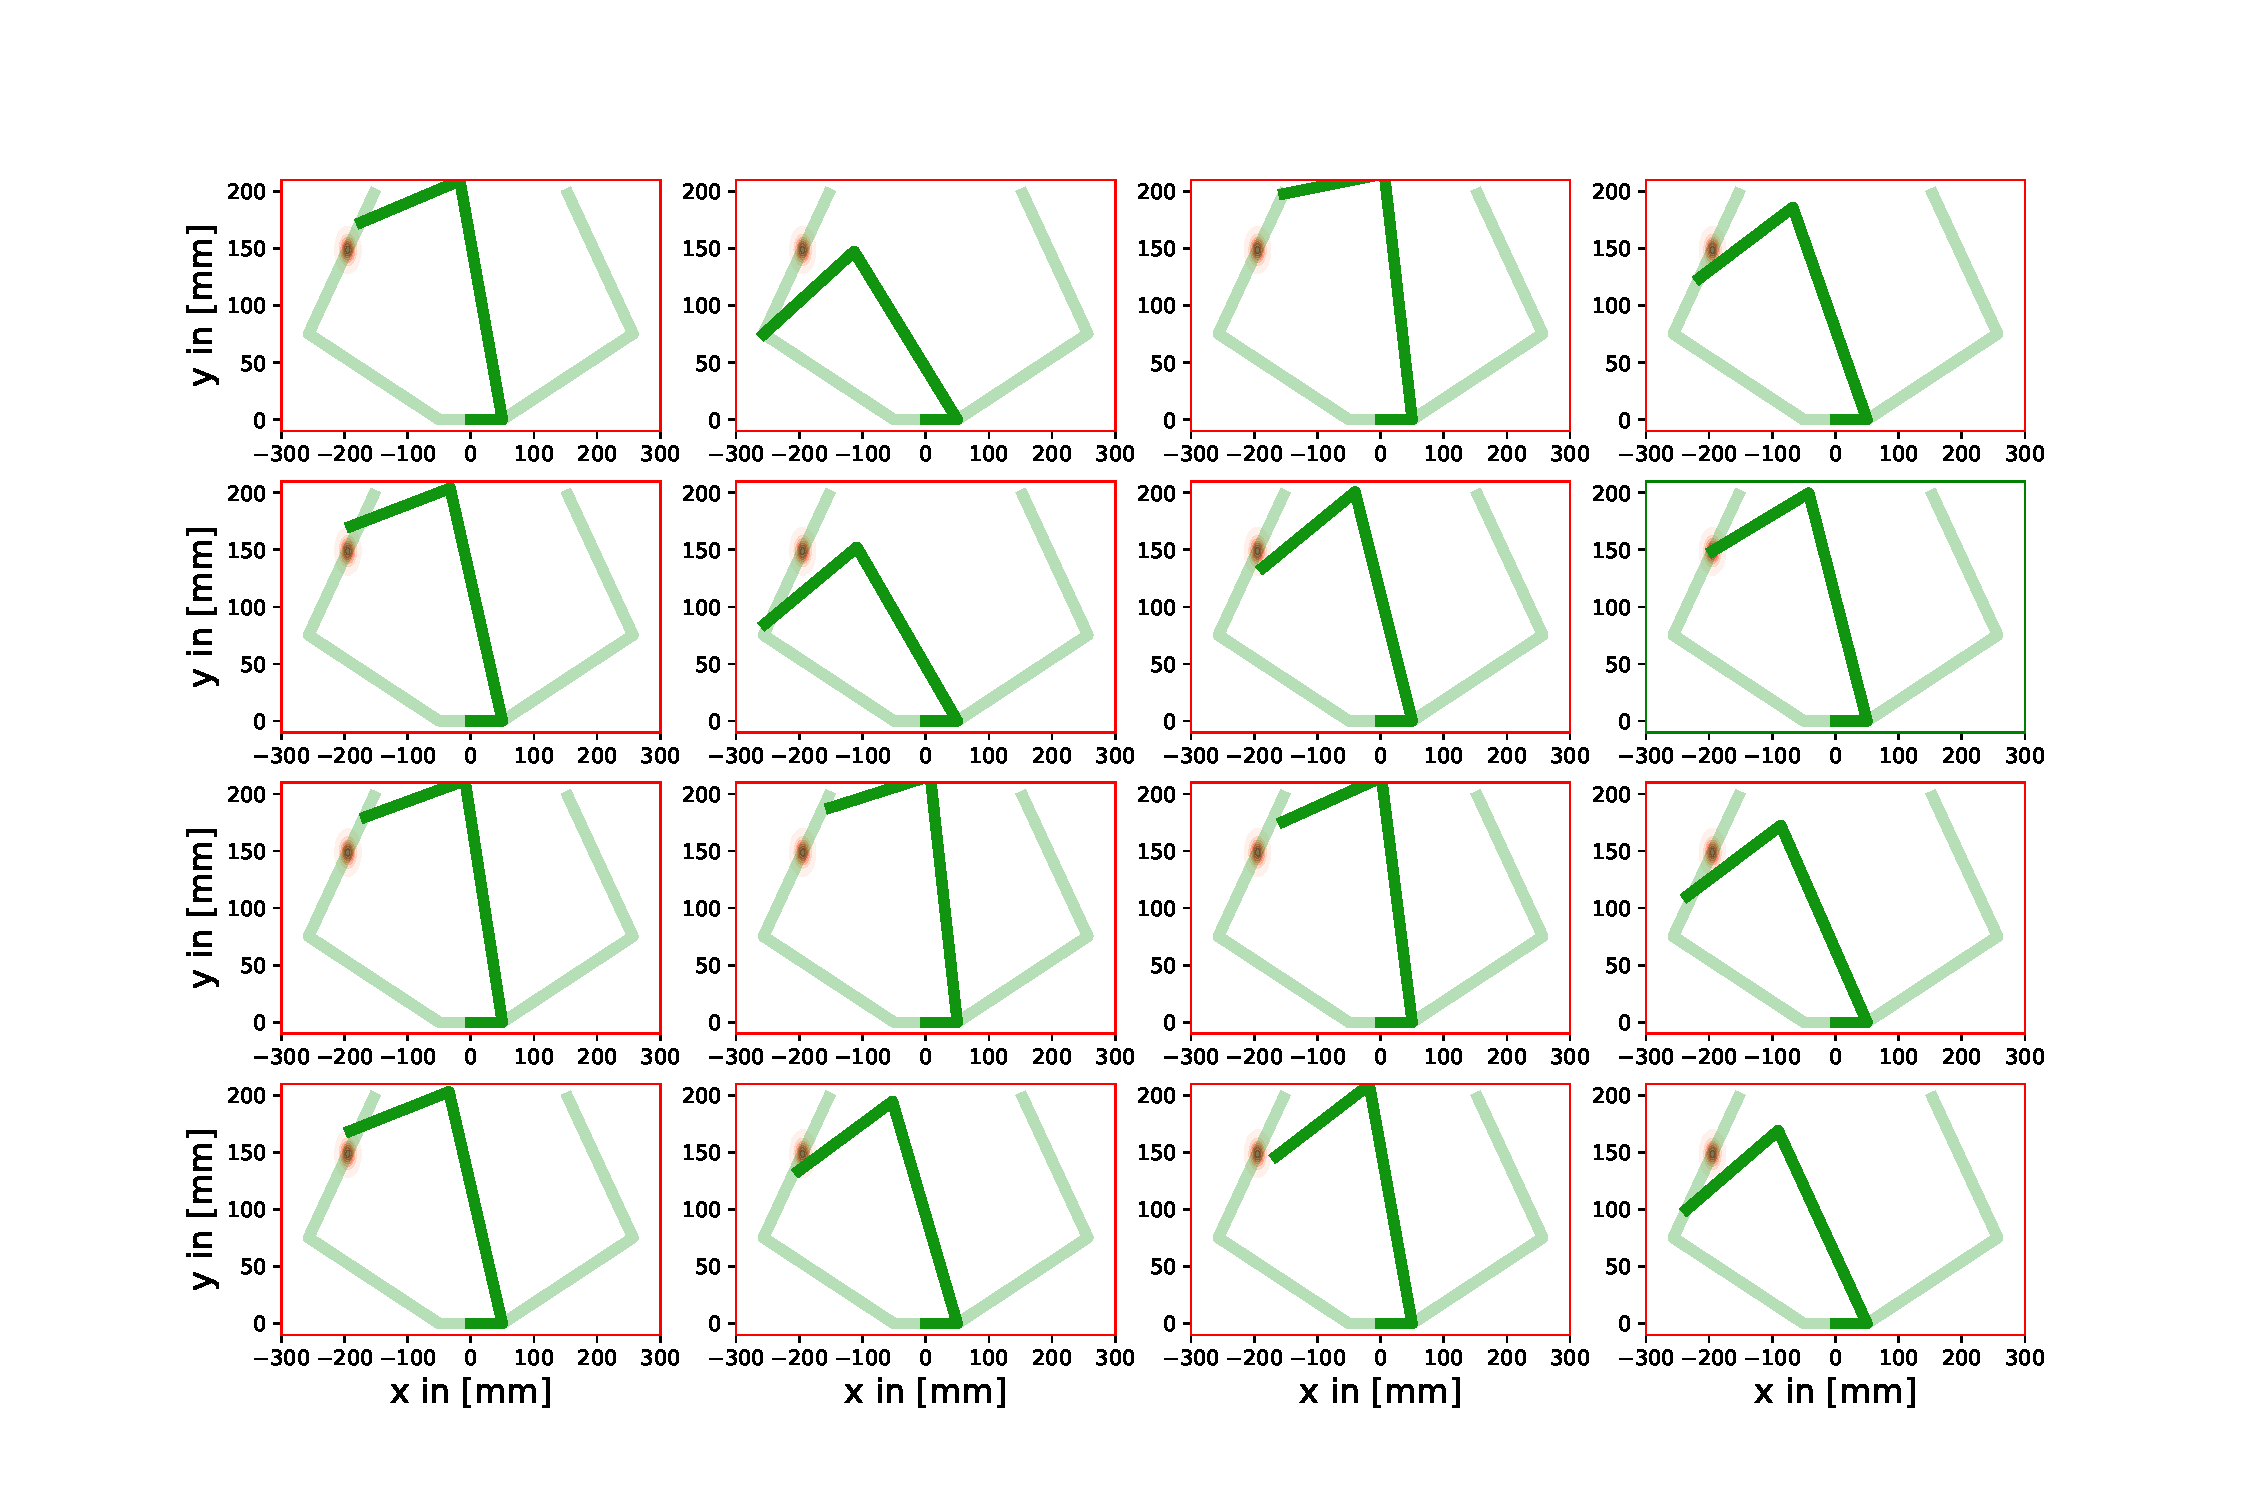
\includegraphics[width=\linewidth]{trajectories}
		\captionof{figure}{Possible trajectories.}
		
	\end{adjustbox}

}


\end{poster}


\end{document}